\documentclass[tikz,convert={outfile=figure2_performance_distribution.png}]{standalone}
\usepackage{pgfplots}
\usepgfplotslibrary{statistics}
\pgfplotsset{compat=1.18}
\begin{document}
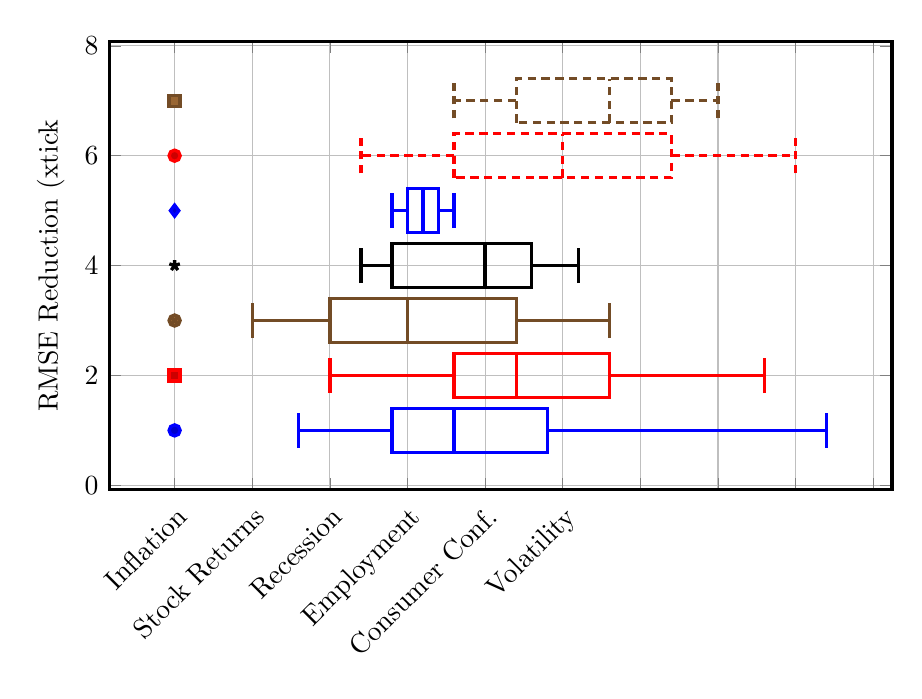
\begin{tikzpicture}
\begin{axis}[
    width=0.95\textwidth,
    height=0.6\textwidth,
    ylabel=RMSE Reduction (%),
    xtick={1,2,3,4,5,6,7},
    xticklabels={GDP, Inflation, Stock Returns, Recession, Employment, Consumer Conf., Volatility},
    xticklabel style={rotate=45, anchor=north east},
    grid=major,
    ymajorgrids=true,
    style={very thick},
]
% GDP: 8, 14, 18, 24, 42
\addplot+[boxplot prepared={
    lower whisker=8, lower quartile=14, median=18, upper quartile=24, upper whisker=42
}] coordinates {(1,0)};
% Inflation: 10, 18, 22, 28, 38
\addplot+[boxplot prepared={
    lower whisker=10, lower quartile=18, median=22, upper quartile=28, upper whisker=38
}] coordinates {(2,0)};
% Stock Returns: 5, 10, 15, 22, 28
\addplot+[boxplot prepared={
    lower whisker=5, lower quartile=10, median=15, upper quartile=22, upper whisker=28
}] coordinates {(3,0)};
% Recession: 12, 14, 20, 23, 26
\addplot+[boxplot prepared={
    lower whisker=12, lower quartile=14, median=20, upper quartile=23, upper whisker=26
}] coordinates {(4,0)};
% Employment: 14, 15, 16, 17, 18
\addplot+[boxplot prepared={
    lower whisker=14, lower quartile=15, median=16, upper quartile=17, upper whisker=18
}] coordinates {(5,0)};
% Consumer Confidence: 12, 18, 25, 32, 40
\addplot+[boxplot prepared={
    lower whisker=12, lower quartile=18, median=25, upper quartile=32, upper whisker=40
}] coordinates {(6,0)};
% Volatility: 18, 22, 28, 32, 35
\addplot+[boxplot prepared={
    lower whisker=18, lower quartile=22, median=28, upper quartile=32, upper whisker=35
}] coordinates {(7,0)};
\end{axis}
\end{tikzpicture}
\end{document}
